\begin{appendix}

%-----------------------------------------------------------------------------
\chapter{Latex in Beispielen}
%-----------------------------------------------------------------------------

%-----------------------------------------------------------------------------
\section{Texthervorhebungen}
%-----------------------------------------------------------------------------

Test {\it Test} {\bf Test} {\tt Test} {\sc Test}

\tiny{Test} \small{Test} \normalsize{Test} \large{Test} \Large{Test}
\LARGE{Test} \huge{Test} \Huge{Test}
\normalsize{Test}

\begin{center}
Das ist ein Text. 
\end{center}

\begin{flushleft}
Das ist ein Text.
\end{flushleft}

\begin{flushright}
Das 
ist 
ein 
Text.

\end{flushright}

\begin{verbatim}
    #ifndef _MYFILENAME_IDL_
    #define _MYFILENAME_IDL_
    
    // some IDL definitions

    #endif /* _MYFILENAME_IDL_ */
\end{verbatim}

\newpage


%-----------------------------------------------------------------------------
\section{Listings}
%-----------------------------------------------------------------------------

\begin{lstlisting}[language=C, caption={Ein einfaches C Programm.}]
#ifndef _MYFILENAME_H_
#define _MYFILENAME_H_

	// some C code here

#endif /* _MYFILENAME_H_ */
\end{lstlisting}

\vspace{1cm}

\lstinputlisting[caption={Ein erstes Java Programm.}]{src/HelloWorld.java}

\newpage

%-----------------------------------------------------------------------------
\section{Aufzählungen}
%-----------------------------------------------------------------------------

\begin{itemize}
  \item eins
  \item zwei
  \item drei
  \begin{itemize}
    \item a
    \item b
    \item c
  \end{itemize}
\end{itemize}

\begin{enumerate}
  \item eins
  \item zwei
  \item drei
\end{enumerate}


\begin{description}
\item[eins] blah
\item[zwei] blah blah
\item[drei] blah blah blah 
\end{description}

\newpage


%-----------------------------------------------------------------------------
\section{Tabellen}
%-----------------------------------------------------------------------------

Es ist leicht möglich auf Tabellen zu verweisen (siehe Tab.~\ref{UserTable}).

\begin{table}[htbp]
\begin{center}
\begin{tabular}{|r||l|c|} 
\hline 
ID 	& Username 	& Password 	\\ 
\hline 
\hline
3 	& Eva 		& xxx 		\\ 
\hline
5 	& Willi 	& xxx 		\\ 
\hline
\end{tabular}
\end{center}
\caption{Eine Beispiel-Tabelle.}
\label{UserTable}
\end{table}


\begin{table}[htbp]
\begin{center}
	\begin{tabular}{|c|c|c|c|c|c|}
	\hline
	\multirow{3}{*}{A} & \multicolumn{2}{c|}{User B} & %
	    \multicolumn{2}{c|}{User C} & \multirow{3}{*}{D}\\
	\cline{2-5}
	 & \multicolumn{2}{c|}{Value} & \multicolumn{2}{c|}{Value} & \\
	\cline{2-5}
	 & B1 & B2 & C1 & C2 & \\
	\hline
	 & & & & & \\
	\hline
	 & & & & & \\
	\hline
	\end{tabular}
\end{center}
\caption{Eine Mehrfach-Zeilen und Mehrfach-Spalten Tabelle.}
\end{table}


\newpage


%-----------------------------------------------------------------------------
\section{Fußnoten und Randnotizen}
%-----------------------------------------------------------------------------
Ein Text kann durch eine Fußnote\footnote{Das ist eine Anmerkung.} ergänzt
werden.

%\marginpar{Das ist eine Randbemerkung.}5

\newpage


%-----------------------------------------------------------------------------
\section{Mathematische Formeln}
%-----------------------------------------------------------------------------

Einfache mathematische Ausdrücke z.B.: $z=a+jb$ können leicht in den
Text eingebettet werden.

\begin{displaymath}
y=\frac{1}{x+1}
\end{displaymath}


\begin{displaymath}
abs = \sqrt{re^2 + im^2}
\end{displaymath}

\begin{displaymath}
\int_{a}^{b} f(x)g(x)dx
\end{displaymath}

\newpage


%-----------------------------------------------------------------------------
\section{Bilder}
%-----------------------------------------------------------------------------

Aus einem Text heraus kann man sich auf ein Bild beziehen (siehe
Abb.~\ref{ComponentDef}), um eine Erklärung zu unterstreichen.

\begin{figure}[htbp]
    \centering
    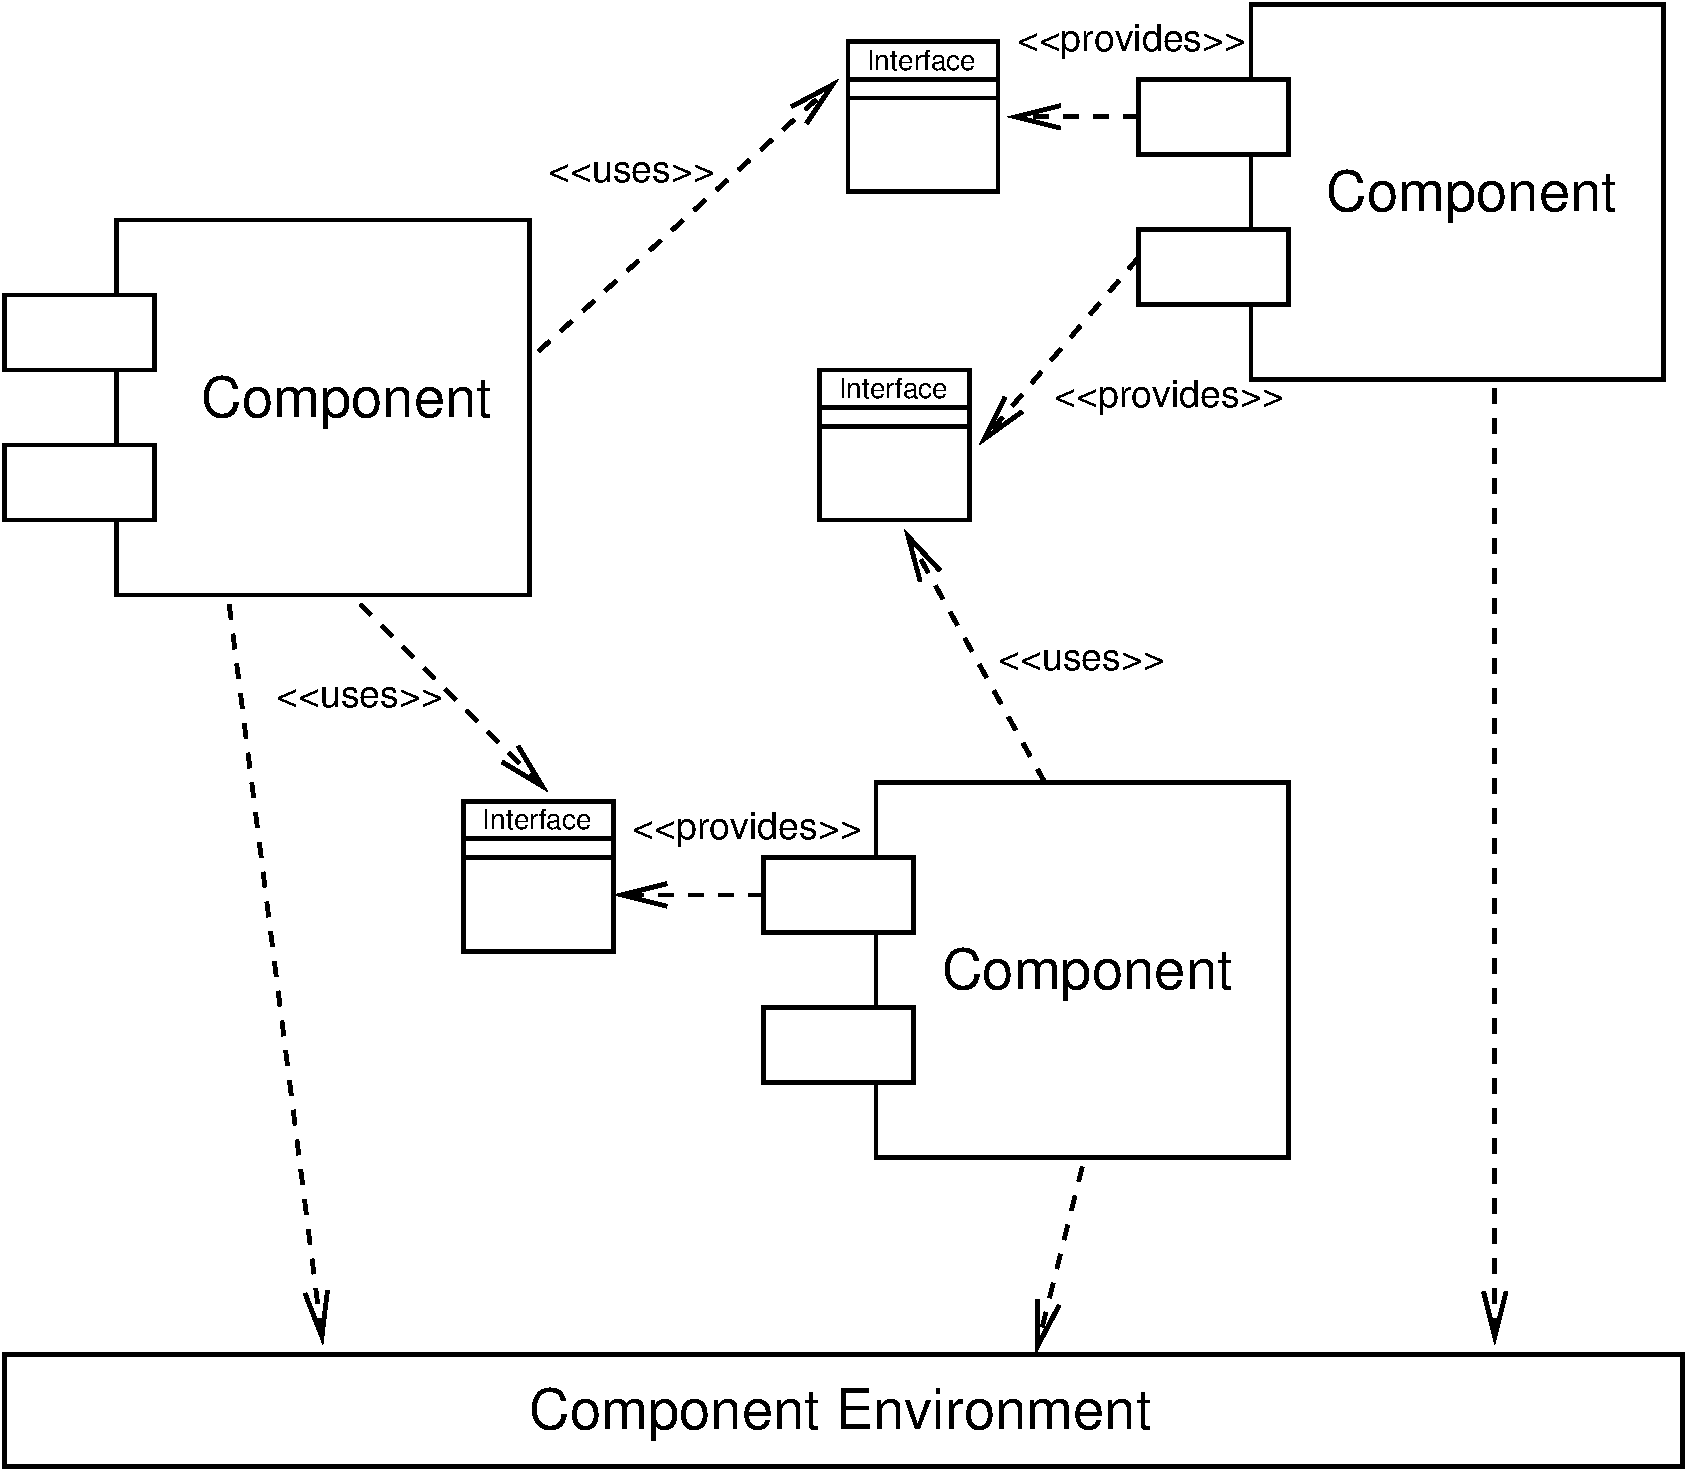
\includegraphics [width=12cm,angle=0] {figures/Environment}
    \caption{A software component is a unit of composition with 
        contractually specified interfaces and explicit context 
		dependencies only.}
    \label{ComponentDef}
\end{figure}


%-----------------------------------------------------------------------------
\section{Zitate}
%-----------------------------------------------------------------------------

Die Voraussetzung für gutes Software Design sind Design Patterns.
Neben dem GoF Buch \cite[S. 190]{Gamma95} gibt es noch zahlreiche andere Bücher
zu diesem Thema \cite[S. 999]{Marinescu02} \cite{dpquiz} \cite{Wick2005}.

\end{appendix}
